\documentclass[12pt]{article}
\usepackage{msc}
\usepackage{amsmath, amssymb}
\usepackage{tikz}
\usetikzlibrary{automata,positioning}
\usepackage{datetime}
\usepackage[utf8]{inputenc}
\usepackage{xspace}

\newdateformat{specialdate}{\twodigit{\THEDAY}.\twodigit{\THEMONTH}.\THEYEAR}

\begin{document}
	
	\title{Diagramm - Element Aufspaltung}
	\author{Timo Bergerbusch}
	\date{\specialdate\today}
	\maketitle
	
	\tableofcontents
	\newpage
	
	\section{Graph}
	\begin{center}
		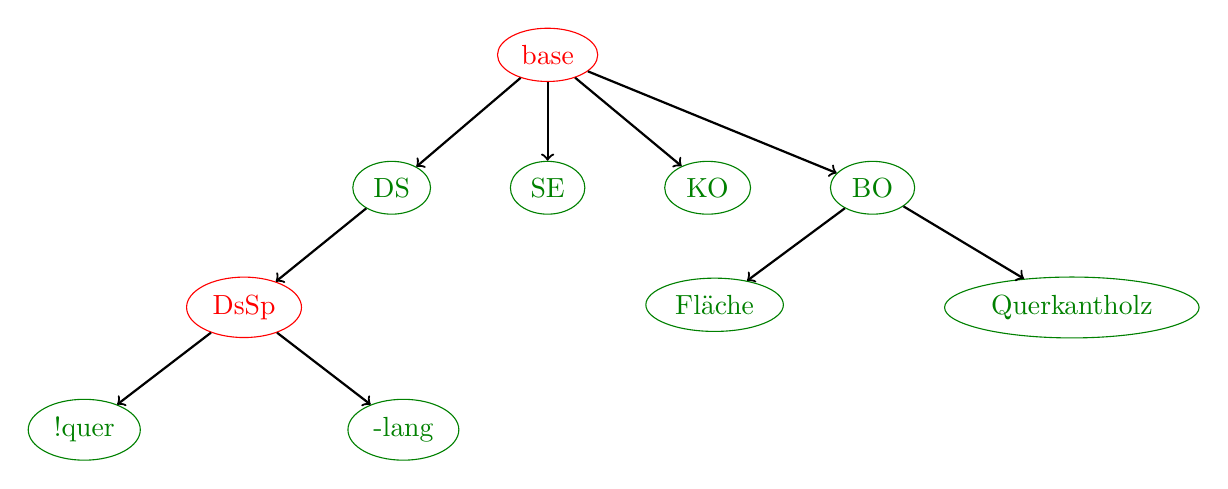
\begin{tikzpicture}[every node/.style={draw,ellipse}, every edge/.style={->, thick, draw}]			
			\node[green!50!black] (deckel){DS};			
			\node[right = of deckel, green!50!black] (seite){SE};
			\node[right = of seite, green!50!black] (kopfstueck) {KO};
			\node[above = of seite, red] (base) {base};
			\node[right = of kopfstueck, green!50!black] (boden) {BO};
			
			\node[below left = of deckel, red] (deckelspange) {DsSp};
			
			\node[below left = of deckelspange, green!50!black] (deckelspangeQuer) {!quer};
			\node[below right = of deckelspange, green!50!black] (deckelspangeLang) {-lang};

			\node[below left = of boden, green!50!black] (bodenFlaeche) {Fläche};
			\node[below right = of boden, green!50!black] (bodenQuer) {Querkantholz};
			
			\draw (base) edge (deckel);
			\draw (base) edge (seite);
			\draw (base) edge (kopfstueck);
			\draw (base) edge (boden);
			
			\draw (deckel) edge (deckelspange);
			\draw (deckelspange) edge (deckelspangeQuer);
			\draw (deckelspange) edge (deckelspangeLang);
			
			\draw (boden) edge (bodenFlaeche);
			\draw (boden) edge (bodenQuer);
		\end{tikzpicture}
	\end{center}
	
	\section{Tabelle}
	\begin{center}
		\begin{tabular}{l|l|l|l|l|l}
			Name 		& Kürzel & Bezeichnungsdetail 	& x-Achse 	& y-Achse 	& z-Achse \\ \hline\hline
			Deckel 		& DE	 &						& Breite 	& Länge 	& Höhe \\
			Deckelspange & DE	 & DeSp !quer			& Länge		& Breite	& Höhe \\
			Deckelspange & DE	 & DeSp -lang			& Breite	& Länge		& Höhe \\
			Seite		& SE	 & 						& Höhe		& Breite	& Länge \\
			Kopfstück	& KO	 & 						& Länge		& Höhe		& Breite \\
			Boden		& BO	 & Fläche				& Breite	& Länge		& Höhe \\
			Boden		& BO	 & Querkantholz			& Breite	& Länge		& Höhe\\
			
			
		\end{tabular}
	\end{center}
	
	\section{Erklärung}
	\subsection{Graph}
		\begin{itemize}
			\item Stellt die Beziehung zwischen Bauteilen da
			\item Bedeutung \color{red}Rot\color{black}: kann so nicht vorkommen\\
				\textbf{Beispiel}: die \color{red}base\color{black}\xspace existiert so \underline{nicht}
			\item Bedeutung \color{green!50!black}grün\color{black}: kann so vorkommen\\
				\textbf{Beispiel}: eine \color{green!50!black}Seite\color{black}\xspace existiert
			\item Zwei Bauteile $B_1,B_2$ sind verbunden ($B_1 \rightarrow B_2$), wenn $B_2$ ein spezielles Baumteil der Form $B_1$ ist\\
			\textbf{Beispiel 1}: Jedes Bauteil ist ein spezielles Base-Bauteil\\
			\textbf{Beispiel 2}: Eine Deckelspange mit dem Zusatz !quer ist eine spezielle Deckelspange
		\end{itemize}
	\subsection{Tabelle}
		\begin{itemize}
			\item[Name:] der Name des Bauteils
			\item[Kürzel:] das Kürzel, welches in der Datei für das Bauteil verwendet wird\\ 
				Hinweis: Deckel und Deckelspangen haben beide das Kürzel \texttt{DE}
			\item[Bez.-D.:] weiter Details in der Spalte "\texttt{Materialgruppe / Werkstoffe}", welche für die weitere Klassifizierung gebraucht werden
			\item[$\eta$-Achse:] die Spalte (\texttt{Länge},\texttt{Breite}, \texttt{Höhe}) die auf der $\eta$-Achse (\texttt{x-Achse}, \texttt{y-Achse}, \texttt{z-Achse}) abgetragen werden soll.\\
			\textbf{Beispiel}: Bei einem Deckel wird die \texttt{Breite} auf der \texttt{x-Achse} abgetragen.
		\end{itemize}
	
	\subsection{Wichtig:}
		Jedes Bauteil, welches vorkommen soll (\color{green!50!black}grün\color{black}\xspace gezeichnet) \color{red}\underline{muss}\color{black}\xspace eindeutig identifizierbar sein. Das Programm kann keine zwei Elemente unterscheiden basierend auf Daten die nicht in der Datei stehen.\\
		Zudem werden alle anderen Anmerkungen in "\texttt{Materialgruppe / Werkstoffe}" ignoriert wenn diese nicht zum identifizieren benötigt werden. So wäre zum Beispiel ein \texttt{!quer} bei einer Seite für das Programm irrelevant.
\end{document}